\documentclass[UTF8, zihao=-4]{ctexart}
\usepackage{graphicx}
\usepackage{geometry}
\usepackage{atbegshi}					 % 用于绝对定位（导入图片）
\usepackage{fancyhdr}
\usepackage{fontspec}                    % 字体管理
\usepackage{titlesec}                    % 标题格式定制
\usepackage{setspace}                    % 行距控制
\usepackage{booktabs}
\usepackage{float}
\usepackage{amsmath}
\usepackage{caption}
\captionsetup[figure]{labelformat=empty}  % 取消图片前缀
\captionsetup[table]{labelformat=empty}   % 取消表格前缀


\usepackage[backend=biber, style=numeric]{biblatex} % 管理参考文献
\usepackage{hyperref} % 添加超链接
\hypersetup{
	colorlinks=true,
	linkcolor=blue,    % 内部链接颜色
	citecolor=blue,     % 引用标记颜色
	urlcolor=blue       % URL颜色
}
\addbibresource{refs.bib}
%正文小四宋体 论文题目三号黑体   一级标题四号黑体居中   二三级标题小四黑体左对齐，单倍行距

\setstretch{1.0} % 严格单倍行距 (1.0倍)
\setlength{\parskip}{0pt}


\title{
	\heiti\zihao{3} % 三号黑体
	\textbf{Craft} \\ % 加粗
	\vspace{0.5em}
	
}

% 一级标题 (section)
\renewcommand{\thesection}{\chinese{section}} % 将 section 序号转为中文数字
\titleformat{\section}
{\centering\heiti\zihao{4}\bfseries} % 四号黑体加粗居中
{\thesection、}{0em}{}

% 二级标题 (subsection)
\renewcommand{\thesubsection}{\arabic{section}.\arabic{subsection}} % 强制使用阿拉伯数字
\titleformat{\subsection}
{\raggedright\heiti\zihao{-4}\bfseries} % 小四黑体加粗左对齐
{\thesubsection}{1em}{}

% 三级标题 (subsubsection)
\titleformat{\subsubsection}
{\raggedright\heiti\zihao{-4}\bfseries} % 小四黑体加粗左对齐
{\thesubsubsection}{1em}{}


% 设置正文字体页边距
\geometry{a4paper, left=3cm, right=2.5cm, top=2.5cm, bottom=2.5cm}
\pagestyle{fancy}  % 激活 fancyhdr 样式
\fancyhf{}         % 清空默认页眉页脚
\fancyfoot[C]{\thepage}  % 在页脚居中显示页码
\renewcommand{\headrulewidth}{0pt}  % 隐藏页眉

\begin{document}
	
	% ---------- 封面页 ----------
	\newgeometry{margin=0cm, nohead, nofoot} % 临时页边距
	\thispagestyle{empty} % 隐藏封面页页码
	
	% 核心修改：使用绝对定位直接覆盖页面
	\AtBeginShipoutNext{%
		\AtBeginShipoutUpperLeft{%
			\put(0,-\paperheight){% 从左上角原点开始定位
				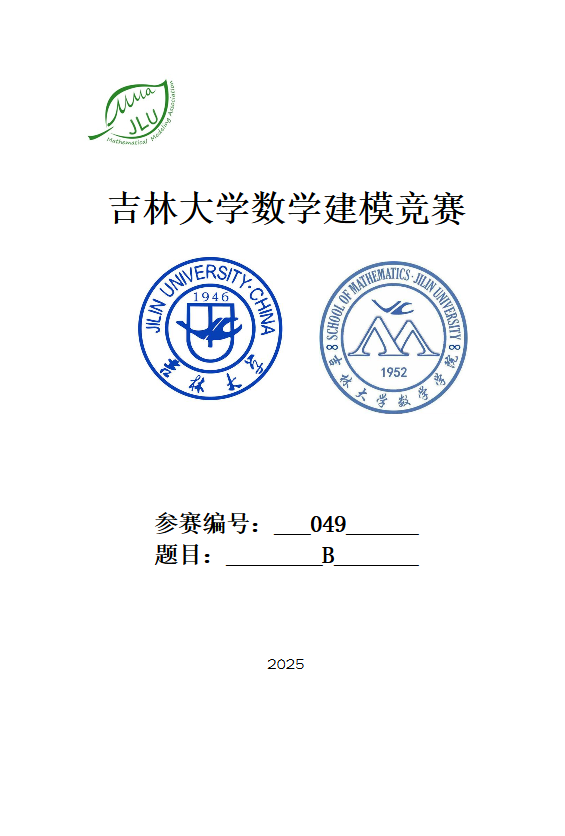
\includegraphics[
				width=\paperwidth,
				height=\paperheight,
				keepaspectratio=false
				]{cover.png}%
			}%
		}%
	}
	\phantom{placeholder}
	\clearpage % 强制结束封面页
	\restoregeometry % 恢复正文字体边距
	
	\maketitle
	\thispagestyle{empty}
	
	% ==================== 自定义摘要环境 ====================
	\newenvironment{abstractwithkeywords}
	{
		\vspace*{2cm} % 顶部间距
		\centering
		{\heiti\zihao{3}\bfseries 摘\quad 要} \\ % 三号黑体加粗
		\vspace{1cm}
		\begin{minipage}{0.9\textwidth} % 控制摘要宽度
			\setlength{\parindent}{2em} % 恢复首行缩进
			\songti\zihao{-4} % 小四宋体正文
		}
		{ % 摘要结束后的关键词部分
		\end{minipage}
		\vspace{1cm}
		
		{\heiti\zihao{-4}\bfseries 关键词：} % 小四黑体加粗
		\heiti\zihao{-4}\bfseries 关键词1；关键词2；关键词3 % 小四宋体
	}
	
	\begin{abstractwithkeywords}
		这里是摘要正文内容。
	\end{abstractwithkeywords}
	
	% ---------- 正文 ----------
	\newpage
	\pagenumbering{arabic}  % 设置页码格式为阿拉伯数字
	\setcounter{page}{1}    % 重置页码为 1（封面页不计数）
	
	\section{问题重述}
	\subsection{问题背景}
	吉林省地处东北地区中部，是新中国汽车工业、电影工业的摇篮。吉林省的教育事业发展势头良好，各学龄阶段教育有很多优势突出、特色鲜明的学校，全省受教育人口比例、升学比例相对较高。可通过较为科学系统的数学方法对吉林省教育事业发展进行分析，为进一步提升教育品质和科学决策水平提供参考依据。
	\subsection{问题要求} 
	问题一：以近几年的吉林省教育事业发展情况，建立数学模型，分别预测未来三年内吉林省义务教育阶段、高中教育阶段、高等教育阶段的在校生人数。
	
	问题二：结合近年来的吉林省人口数据，分析吉林省人口与本省各阶段教育之间的影响。
	
	问题三：为提振吉林省经济发展，希望通过加大对教育事业的投入吸引人才，减少人口外流。请结合近几年的吉林省教育经费数据，对未来三年内吉林省各项教育经费做出合理预算，为提高各阶段教育水平提出合适的策略分析。
	
	\section{符号说明}
	\begin{tabular}{@{}p{6cm} p{8cm}@{}}
		\toprule
		\textbf{符号} & \textbf{说明} \\
		\midrule
		$X_1$        & 出生率/\% \\
		$X_2$		 & 死亡率/\% \\
		$X_3$		 & 人口自然增长率/\% \\
		$X_4$		 & 城镇化率/\% \\
		$X_5$		 & 年末常驻人口数/万人 \\
		$X_6$		 & 义务教育学校数  \\
		$X_7$		 & 高中教育学校数  \\
		$X_8$		 & 高等教育学校数  \\
		$Y^{(1)}$    & 义务教育在校生人数/万人 \\
		$Y^{(2)}$    & 高中教育在校生人数/万人 \\
		$Y^{(3)}$    & 高等教育在校生人数/万人 \\
		$\beta_n$ 	 & 多元线性回归系数  \\
		\bottomrule
	\end{tabular}
	
	\section{问题分析}
	针对问题一：考虑到有准确的在校生人数历史数据\autocite{tjnj}（整理后如下图3-1），可以选择建立{\bfseries 时间序列模型}，因其无需复杂因果分析且适合短期预测。但通过计算我们发现义务教育和高等教育的相关数据不满足时间序列的建立条件，即时间序列{\bfseries 不平稳}，于是建立{\bfseries 多元线性回归模型}。
	\begin{figure}[H]
		\centering
		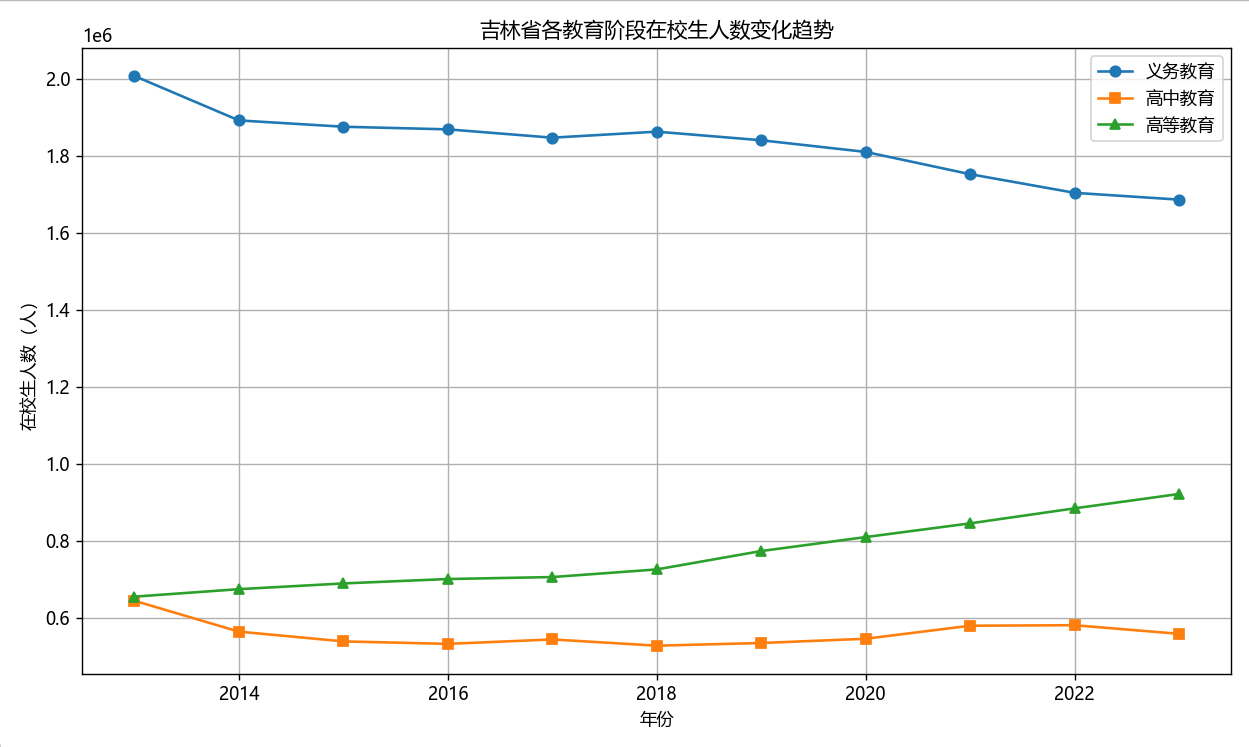
\includegraphics[width=0.5\textwidth]{../图片/在校生人数变化趋势.png}
		\caption{\zihao{6}图3-1}
	\end{figure}
	
	针对问题二：
	
	
	\section{问题一模型的建立与求解}
	\subsection{数据分析与处理}
		由分析，我们将建立多元线性回归方程，因此各自变量间的相关性应尽可能弱且与在校生人数相关性强。故建立模型方程为：
		
		\[
		Y^{(i)} = \beta_0 + \sum_{j=1}^{8}\beta_jX_j
		\]
		
		我们采用最小二乘法估计系数向量$\beta$:
		
		\[
		\hat{\beta} = (\textbf{X}^T\textbf{X})^{-1}\textbf{X}^T\textbf{Y}
		\]
		
		其中\textbf{X}为自变量$X_i(i=1,...,8)$与年份$t$的设计矩阵，\textbf{Y}为因变量向量
		
		由此还注意到我们还需要2025-2027年的$X_1$,...,$X_8$。观察历年相关数据\autocite{tjnj}（整理如图4-1至4-3）
		\begin{figure}[H]
			\centering
			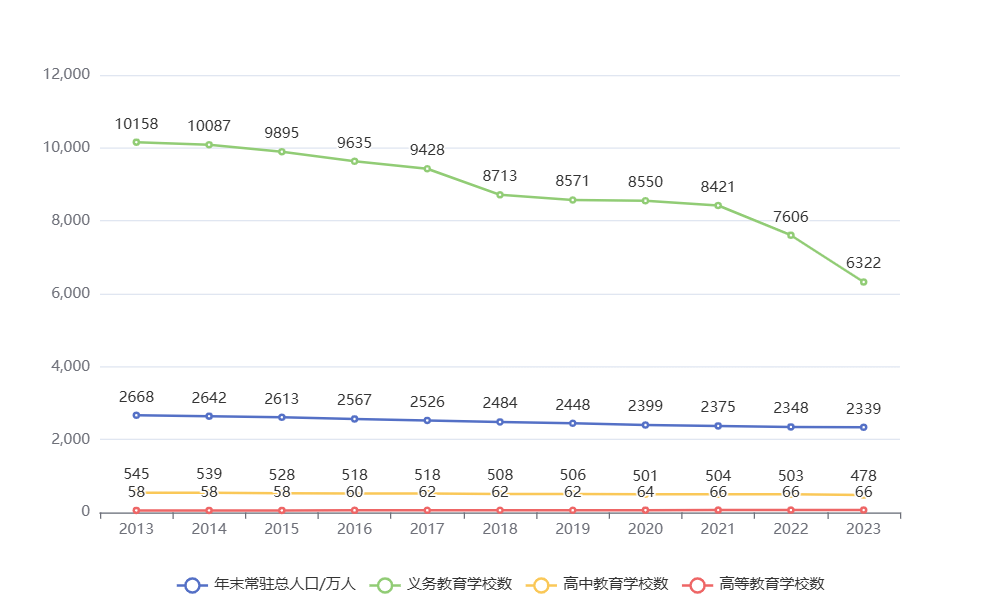
\includegraphics[width=0.7\textwidth]{../图片/4-1.png}
			\caption{\zihao{6}图4-1}
			\label{fig:4a}
		\end{figure}
		\begin{figure}[H]
			\centering
			\begin{minipage}[b]{0.48\textwidth}
				\centering
				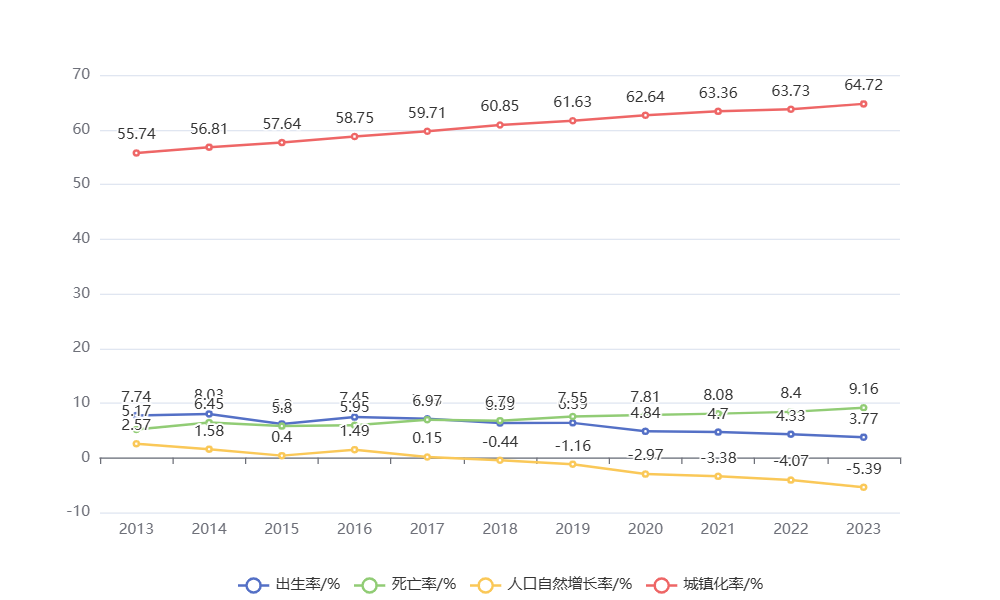
\includegraphics[width=\textwidth]{../图片/4-2.png}
				\caption{\zihao{6}图4-2}
				\label{fig:4b}
			\end{minipage}
			\hfill
			\begin{minipage}[b]{0.48\textwidth}
				\centering
				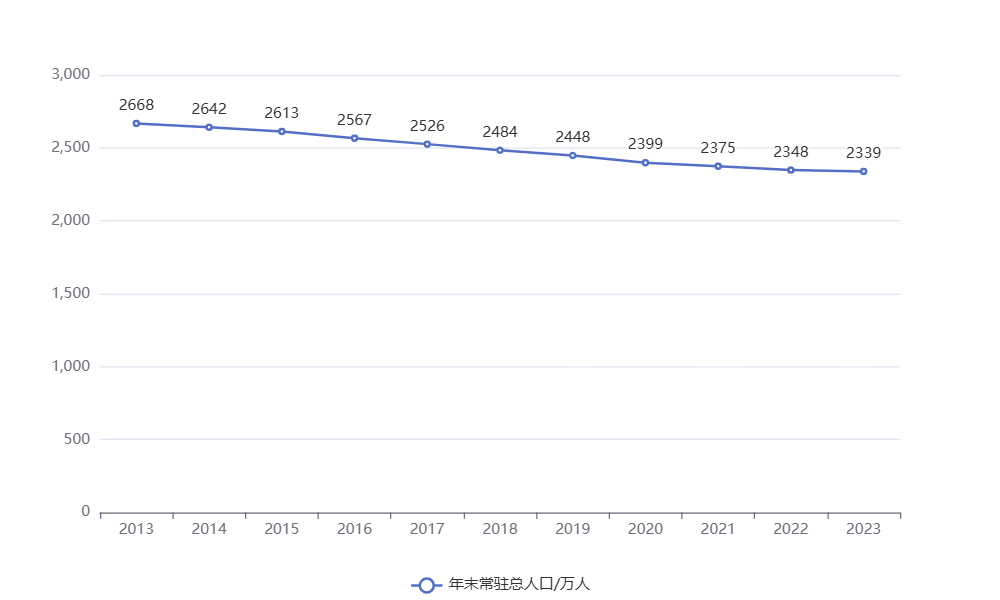
\includegraphics[width=\textwidth]{../图片/4-3.png}
				\caption{\zihao{6}图4-3}
				\label{fig:4c}
			\end{minipage}
		\end{figure}
		
		可以发现各变量变化趋势呈线性，故对各变量线性拟合,可得其预测值$\hat{X}_{i,future}$的时间序列线性回归方程：
		
		\[
		\hat{X}_{i,future} = \alpha_0 +\alpha_1t + \epsilon
		\]
		
		其中$\alpha_0$为常数，$\alpha_1$为年际变化率，$\epsilon$为随机误差。
		参数估计方法目标函数为：
		
		\[
		\min_{\alpha_0,\alpha_1}\sum_{i=1}^{8}[X_i - (\alpha_0+\alpha_1t_i)]^2
		\]
		
		可解得：
		
		\[
		\hat{\alpha}_1 = \frac{\sum(t_i - \bar{t})(X_i - \bar{X})}{\sum(t_i-\bar{t})^2}, \hat{\alpha}_0 = \bar{X} - \hat{\alpha}_1\bar{t}
		\]
		
		这样我们就能得到变量$X_1,...,X_8$的预测值,结果如图4-4至4-6：
		\begin{figure}[H]
			\centering
			\begin{minipage}[b]{0.7\textwidth}
				\centering
				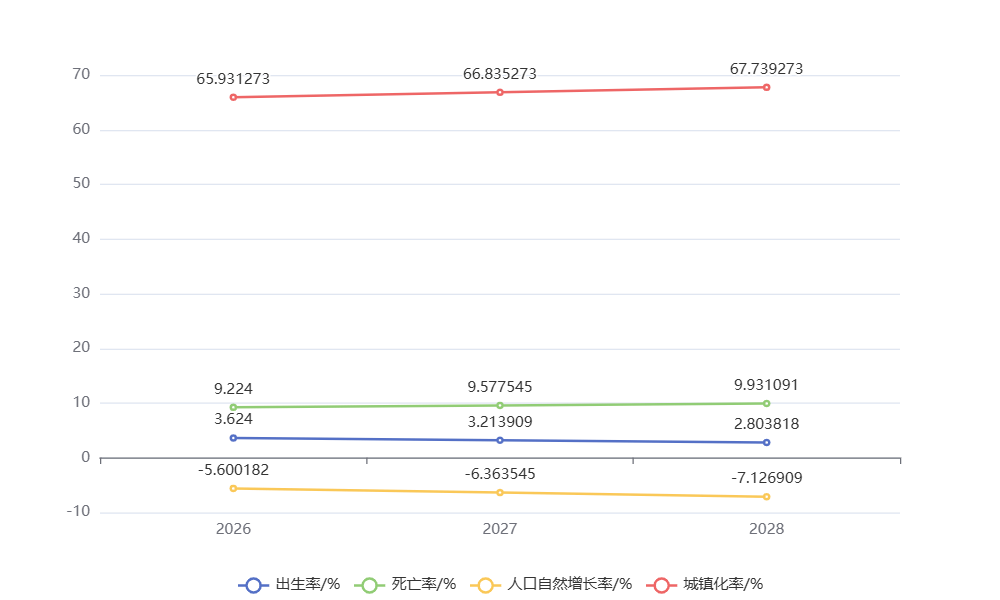
\includegraphics[width=\textwidth]{../图片/4-4.png}
				\caption{\zihao{6}图4-4}
				\label{fig:4d}
			\end{minipage}
		\end{figure}
		\begin{figure}[H]
			\centering
			% 第二张图
			\begin{minipage}[b]{0.48\textwidth}
				\centering
				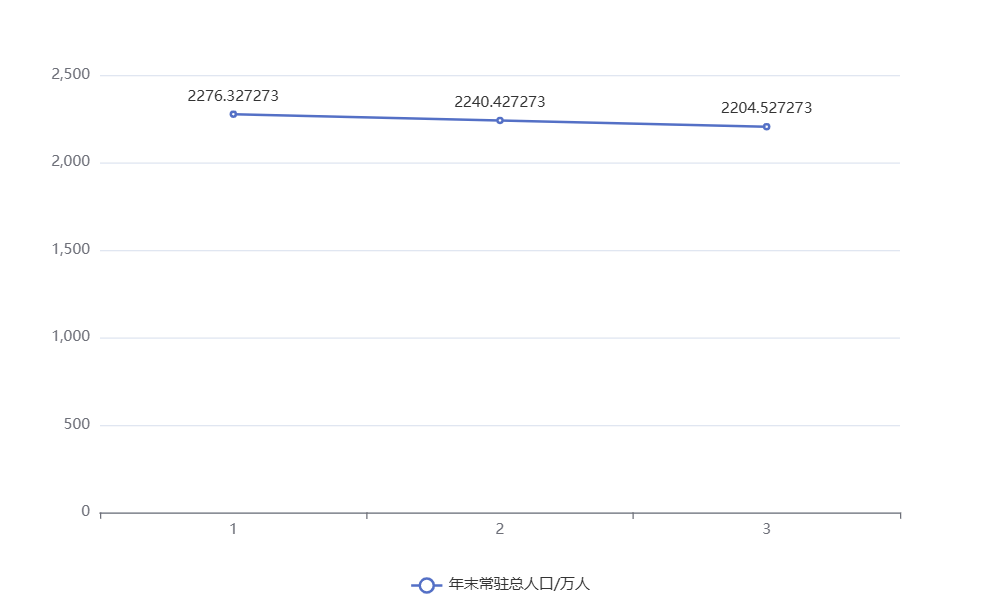
\includegraphics[width=\textwidth]{../图片/4-5.png}
				\caption{\zihao{6}图4-5}
				\label{fig:4e}
			\end{minipage}
			\hfill % 填充水平间距
			% 第三张图
			\begin{minipage}[b]{0.48\textwidth}
				\centering
				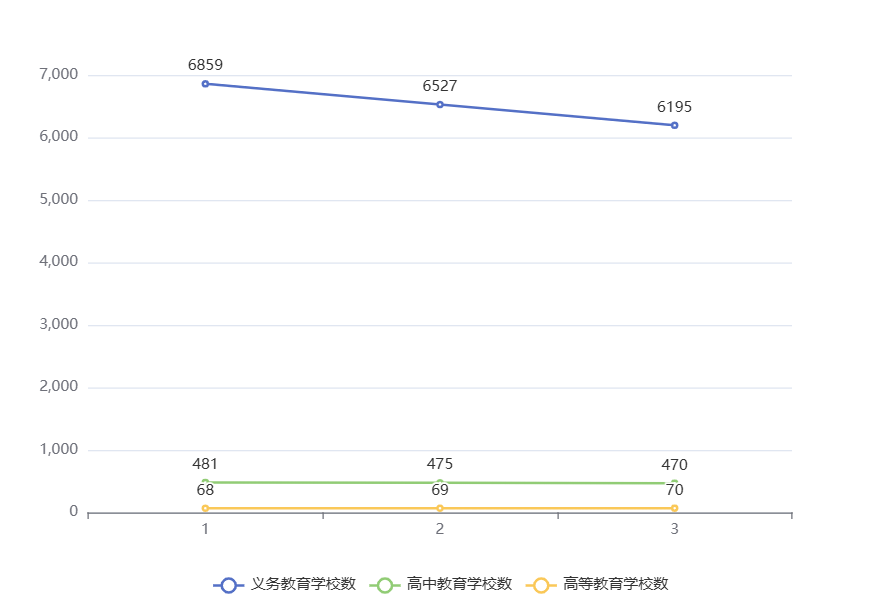
\includegraphics[width=\textwidth]{../图片/4-6.png}
				\caption{\zihao{6}图4-6}
				\label{fig:4f}
			\end{minipage}
			
		\end{figure}
	
	\subsection{建模求解}
		由上述分析我们知道:
		\[
		\hat{Y}^{(i)} = \hat{\beta}_0 + \sum_{j=1}^{8}\hat{\beta}_j\hat{X}_j
		\]
		我们这么来考察参数的估计：
		\begin{itemize}
			\item 残差是否近似正态分布
			\item 异方差检验，Breusch-Pagan检验统计量：$LM=n \times R^2$
			\item 辅助回归拟合优度$R^2$：
			\[
				R^2 = 1 - \frac{\sum(Y_i - \hat{Y}_i)^2}{\sum(Y_i - \bar{Y})^2}
			\]
			\item 调整$R^2$：
			\[
			\bar{R}^2 = 1 - (1-R^2)\frac{n - 1}{n-k-1}
			\]
		借助statsmodels.api库的OLS函数，线性回归系数的计算结果如下：
		\begin{table}[H]
			\begin{minipage}[b]{0.3\textwidth}
				\centering
			\begin{tabular}{@{}c c@{}}
				\toprule
				\textbf{符号} & \textbf{值} \\
				\midrule
				$\beta_0$ & 2707.2656\\
				$\beta_1$ & -997.6949\\
				$\beta_2$ & 1000.0800\\
				$\beta_3$ & 1001.7301\\
				$\beta_4$ & -22.0836\\
				$\beta_5$ & -0.3513\\
				$\beta_6$ & 0.0055\\
				$\beta_7$ & -1.0721\\
				$\beta_8$ & 2.8807\\
				\bottomrule
			\end{tabular}
			\caption{\zihao{6}$Y^{(1)}\text{的方程参数}$}
			\end{minipage}
			\begin{minipage}[b]{0.3\textwidth}
				\centering
			\begin{tabular}{@{}c c@{}}
				\toprule
				\textbf{符号} & \textbf{值} \\
				\midrule
				$\beta_0$ & 987.3537\\
				$\beta_1$ & -301.3441\\
				$\beta_2$ & 301.4557\\
				$\beta_3$ & 301.0550\\
				$\beta_4$ & -11.0388\\
				$\beta_5$ & -0.1484\\
				$\beta_6$ & -0.0024\\
				$\beta_7$ & -0.1035\\
				$\beta_8$ & 2.9065\\
				\bottomrule
			\end{tabular}
			\caption{\zihao{6}$Y^{(2)}\text{的方程参数}$}
			\end{minipage}
			\begin{minipage}[b]{0.3\textwidth}
				\centering
			\begin{tabular}{@{}c c@{}}
				\toprule
				\textbf{符号} & \textbf{值} \\
				\midrule
				$\beta_0$ & 69.1046\\
				$\beta_1$ & 208.6819\\
				$\beta_2$ & -209.2665\\
				$\beta_3$ & -211.1939\\
				$\beta_4$ & 0.3707\\
				$\beta_5$ & -0.0291\\
				$\beta_6$ & -0.0043\\
				$\beta_7$ & 0.2464\\
				$\beta_8$ & -0.4878\\
				\bottomrule
			\end{tabular}
			\caption{\zihao{6}$Y^{(3)}\text{的方程参数}$}
			\end{minipage}
			\end{table}
		\clearpage
		最后，我们得出对未来三年在校生人数的预测如下：
			\begin{figure}[H]
			\centering
			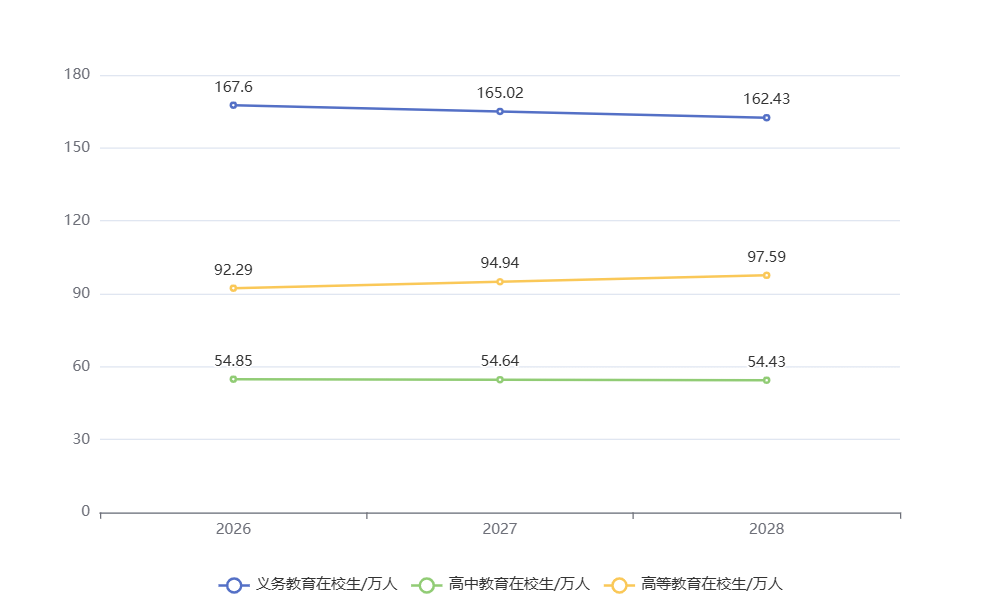
\includegraphics[width=0.7\textwidth]{../图片/4-7.png}
			\caption{\zihao{6}图4-7}
		\end{figure}
		
		\end{itemize}

\defbibheading{bibliography}[\bibname]{%
	\section*{#1} % 不编号的 section
}
\renewcommand{\bibname}{参考文献} % 定义标题名称
\printbibliography
\end{document}